\documentclass[12pt]{article}
\usepackage{graphicx}
\usepackage{amsmath}
\usepackage[margin=1in]{geometry}
\newcommand{\BigO}[1]{\ensuremath{\operatorname{O}\bigl(#1\bigr)}}

\begin{document}

{\Large
\textbf{Computational Physics HW 1}

\textbf{Joseph Yuan}
}

\section*{Problem 3.7: The Mendelbrot Set}

The Mendelbrot set contains complex numbers $\{c_i\}$.  A complex number $c$ exists in the set if it satisfies the condition that $|z_n| < 2$ where $z_n$ is defined by the recursive relationship $z_n+1 = z_n^2 + c$ and $n$ is taken to infinity starting with $z_0 = 0$.

For computational purposes it is necessary to approximate infinity with a reasonably high value for the problem.  We express the complex number as $c = x + iy$.  It can be seen that solutions are bounded within $-2 \le x,y \le 2$ as $z_1 = c$ which for any value outside that range will violate the condition.

\begin{equation}
\begin{array}{rcl}
|z_1|&=&|c|\\
&=&\sqrt{cc^*}\\
&=&\sqrt{(x+iy)(x-iy)}\\
&=&\sqrt{(x^2+y^2)}
\end{array}
\end{equation}

If we consider the edge cases where x or y leaves $[-2,2]$ by an amount $\delta > 0$.  For an example we will take $(x,y) = (2+\delta,0)$.

\begin{equation}
\begin{array}{rcl}
|z_1|&=&\sqrt{(2+\delta)^2} \\
|z_1|&=&2+\delta > 2
\end{array}
\end{equation}

Similarly for  $(x,y) = (-2-\delta,0)$.

\begin{equation}
\begin{array}{rcl}
|z_1|&=&\sqrt{(-2-\delta)^2} \\
|z_1|&=&\sqrt{[(-1)(2+\delta)]^2} \\
|z_1|&=&\sqrt{[(2+\delta)]^2} \\
|z_1|&=&2+\delta > 2
\end{array}
\end{equation}

By symmetry of $|z_1|$ the same applies at the bounds for $y$.  We can see from the form of $|z_1|$ that this creates a circular bound with radius 2.

We create an $N\times N$ grid of points to discretized our region.  Each point representing a unique value for $c = x + iy$ for N steps in x from -2 to 2 and N steps in y from -2 to 2.  We also use this variable N as the number of iteration steps to determine inclusion of $c$ in the Mendelbrot set.  As we increase N we can see an increase in definition of the set.  We visualize our results by treating them first as a bitmap pixelating the data with black pixels for included and white pixels for excluded points.

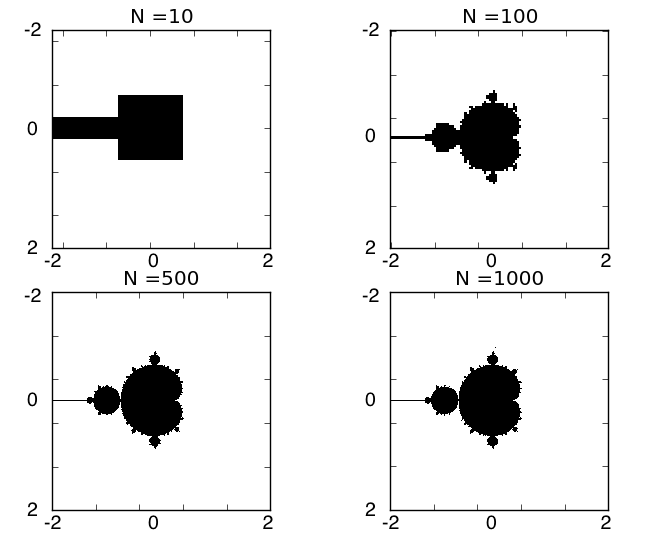
\includegraphics{rv_bw_fourplot.png}

An interesting way to display the set is to scale the data by the number of iterations until the condition is violated.  The data can then be scaled logarithmically to display the structure based on rate of divergence showing what is referred to as the fine structure of the set.  Harkening back to the circular form of $|z_1|$ we can see here the circular boundary this creates.

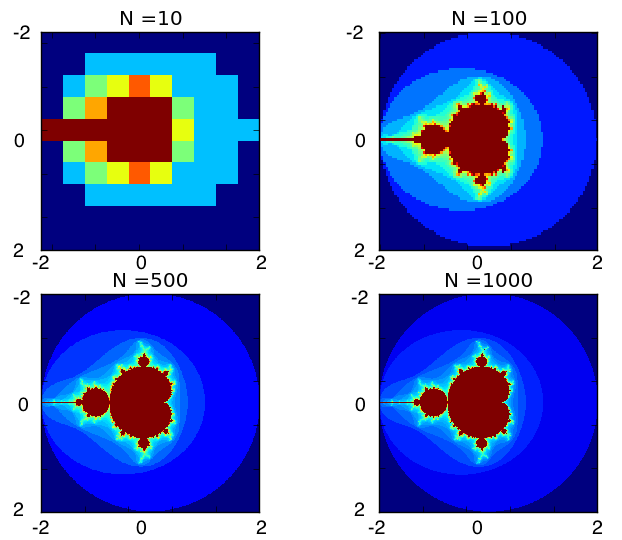
\includegraphics{rv_color_log_fourplot.png}

The algorithm implemented here utilizes numpy's array data structures.  We can create a 2D array for all the discretized values of $c$.  The condition can be implemented as a for loop with an exit upon violation of the condition.  This gives an upper bound on valuation time of $\BigO{N^3}$ for points that do not diverge in N steps the larger.  There are some simple steps we can take to better the performance here.  In the form we are displaying the results the symmetry about the real ($x$) axis. We can utilize this fact and calculate half the set in the complex plane $y \in [-2,0]$ and reflect that over the real line to fill in the other half.  This gives an obvious speed up as one dimension can be reduced in half giving a new upper bound of $\BigO{N^3/2}$.  The actual performance is much better than this estimate and characteristic times could be determined in further investigation.
  
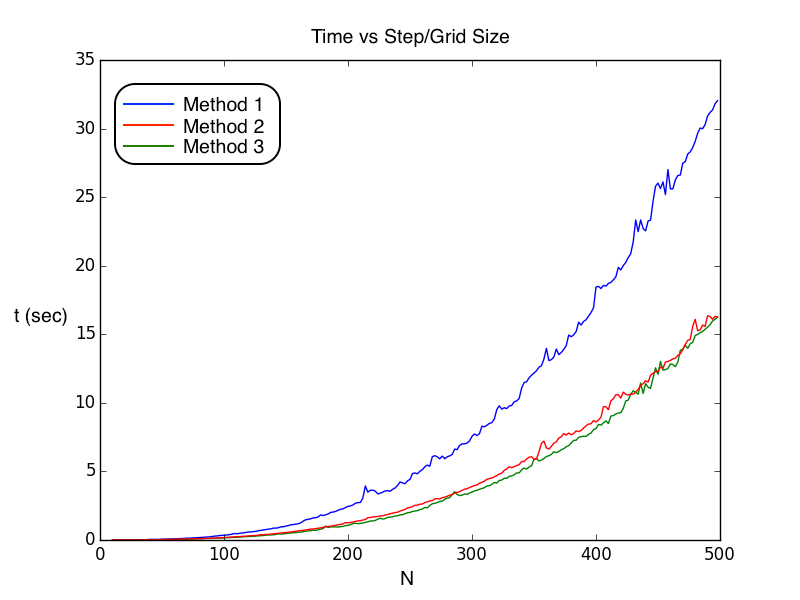
\includegraphics[scale=.8]{time_dep.png}

The above plot shows time dependance of algorithms (color in PDF).  The performance increases are evident by making the above improvements.  The plots of the set in this report were created with the more efficient algorithm and therefore are centered about the zero point and include the set of real numbers which exist in the set for $-2 < x < \frac{1}{4}$.  Method 1 simply performs the limit analysis on each point in the space.  Method 2 calculates the limit individually on each point in half of the complex plane and stores the result in that position and its reflection.  Method 3 creates a half sized matrix ($N \times N/2)$ and lets numpy handle the vectorized calculation.  Afterwards the result and its reflection across the real line are then simply placed in an $N \times N$ matrix.

\section*{Problem 3.8 Least-squares fitting and the \\photoelectric effect}

When comparing phenomena to theory we attempt to see how collected data matches up to theoretical equations.  If the equation predicts linear behavior we attempt to fit a line by finding the parameters of the general linear equation:

\begin{equation}
y = mx + b
\end{equation}

where $y$ and $x$ are the data points, $m$ is the slope, and $b$ is the y-intercept.  This strategy finds the line which minimizes the sum of the vertical distances from each point to the line:

\begin{equation}
\chi^2 = \sum^{N}_{i=1}(mx_i + b - y_i)^2
\end{equation}

We can then minimize and create a set of linear equations by differentiating this sum with respect to $m$ and $c$ and setting equal to zero.  Once solved this set gives results as:

\begin{equation}
m = \frac{N\sum^N_{i=1}x_iy_i - (\sum^N_{i=1}x_i)(\sum^N_{i=1}y_i)}{N\sum^N_{i=1}x_i^2 - (\sum^N_{i=1}x_i)^2}
\end{equation}
\begin{equation}
c = \frac{(\sum^N_{i=1}x_ix_i)(\sum^N_{i=1}y_i) - (\sum^N_{i=1}x_i)(\sum^N_{i=1}x_iy_i)}{N\sum^N_{i=1}x_i^2 - (\sum^N_{i=1}x_i)^2} 
\end{equation}

We can calculate these sums individually and the denominator of both terms a single time to lower processing time and evaluate the parameters which minimize the sum of the vertical distances.  This implementation reads the data into numpy arrays.  The arrays are then summed appropriately to find $m$ and $c$.

To view the data alone we can plot it:

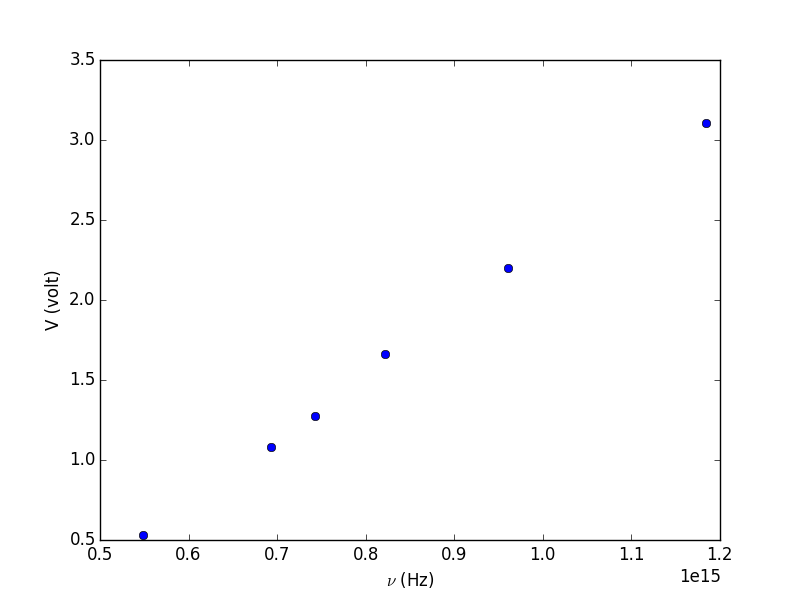
\includegraphics[scale=.8]{reg_a.png}

After calculation of the fit parameters we can plot the line they create at the x values of our data:

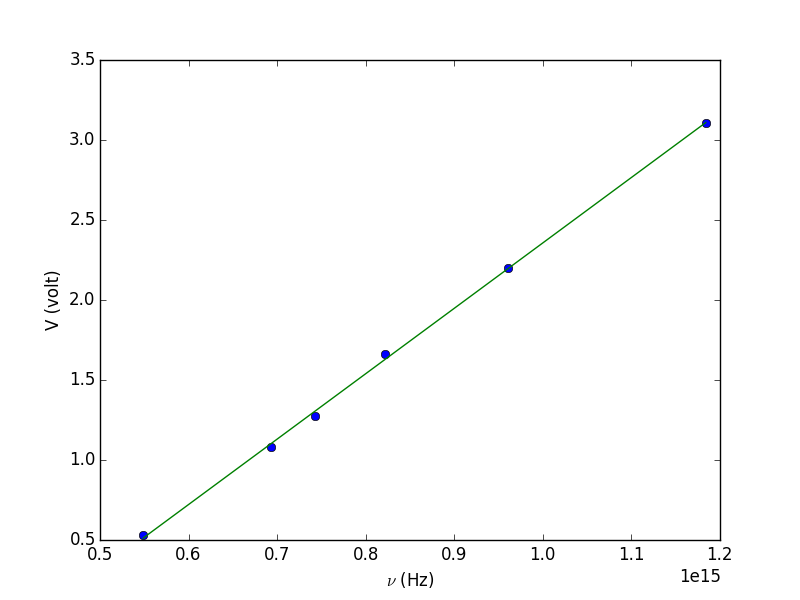
\includegraphics[scale=.8]{reg.png}

From comparison to the photoelectric effect equation we can compare $\frac{h}{e}$ to our slope $m$ to obtain a value of planck's constant $h$.  We use the accepted value of the charge of an electron $e = 1.602 \times 10^{-19} C$ to find $h = 6.5493 \times 10^{-34}$.  This gives a relative error of $1.158\%$ when compared to the current accepted value of $h = 6.6261\times 10^{-34}$

\end{document}